\documentclass[a4paper]{article}
\usepackage[utf8x]{inputenc}
\usepackage[lastexercise]{exercise}
\usepackage{color}
\usepackage{amssymb}
\usepackage[absolute]{textpos} 
\usepackage{verbatim}
\usepackage{ifthen}
\usepackage{tikz}
\usepackage{xkeyval,calc,listings,fp}
\usetikzlibrary{calc}
\usetikzlibrary{positioning}

\renewcommand\ExerciseName{Exercice}
\renewcommand{\AnswerHeader}{\medskip\centerline{\textbf{Solution de
                        l'\ExerciseName  \ExerciseHeaderNB}\smallskip}}
\newenvironment{CAnswer}{\color{red}\begin{Answer}}
                        {\end{Answer}}

\title{Prolog - TP4\\Le problème des n reines}
\date{}

\begin{document}
\maketitle
\begin{textblock*}{4cm}(10mm,10mm)
\begin{Large}ESIAL 3A IL LE\end{Large}
\end{textblock*}
\begin{textblock*}{3cm}(160mm,10mm)

\includegraphics[width=\textwidth]{../../ESIAL.pdf}
\end{textblock*}

\section*{Le problème}
Soit n un entier positif non nul. On souhaite disposer n reines sur un damier
carré de n cases de côté de manière à ce qu'aucune reine ne puisse en prendre
une autre. Une reine peut prendre toute pièce se trouvant sur la même ligne
horizontale, verticale ou diagonale qu'elle.
Une solution possible avec n = 4 :
\begin{center}
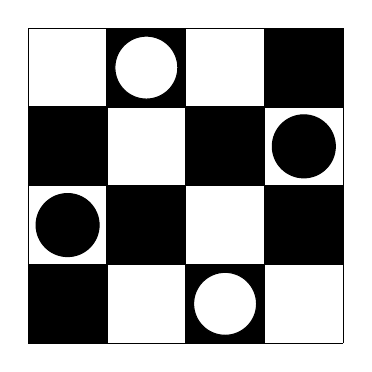
\begin{tikzpicture}[node distance=1.5em]
 \pgfpathgrid[step={\pgfpoint{1cm}{1cm}}]
  {\pgfpoint{0cm}{0cm}}{\pgfpoint{4cm}{4cm}}
 \pgfusepath{stroke}
 \draw[fill=black] (0,0) rectangle  (1,1)
                         rectangle  (2,2)
                         rectangle  (3,3)
                         rectangle  (4,4)
                   (0,2) rectangle  (1,3)
                         rectangle  (2,4)
                   (2,0) rectangle  (3,1)
                         rectangle  (4,2);
\draw[fill=black] (0.5, 1.5) circle (4mm)
                  (3.5, 2.5) circle (4mm);
\draw[fill=white] (1.5, 3.5) circle (4mm)
                  (2.5, 0.5) circle (4mm);
\end{tikzpicture}
\end{center}
Dans ce TP, nous vous proposons d'utiliser le mécanisme de programmation par
contraintes de Prolog. (On pourrait résoudre le problème d'une autre manière).

\section*{Le codage du plateau}
Il existe plusieurs représentation possible du plateau. On pourrait prendre
une liste de $n*n$ entiers où chaque entier vaut 1 lorsqu'il y a une reine 
dans la case correspondante, 0 sinon.

Le damier de l'exemple serait représenté par la liste:
\begin{verbatim}
[0,1,0,0,
 0,0,0,1,
 1,0,0,0,
 0,0,1,0]
\end{verbatim}
Cependant on peut choisir une manière plus compacte de représenter le plateau.
On sait qu'il ne peut pas avoir plus d'une reine par ligne et qu'il y a donc 
exactement une reine par ligne puisqu'il y a n reines et n lignes. On peut
donc représenter le plateau par liste de $n$ entiers où chaque entier 
représente la position de la reine sur la ligne correspondante.

Le plateau de l'exemple est donc codé de la manière suivante :
\verb$[2,4,1,3]$

\begin{Exercise}[title={Problème des n tours}]
Pour l'instant nous ne considérerons pas le cas de reines sur la même 
diagonale. Ecrire un prédicat \verb$n_tours(N,Solution)$ qui instanciera
\verb$Solution$ à une liste de $n$ entiers représentant les tours sur le
plateau tel qu'aucune d'elles ne soit sur la même ligne.

Indication : le prédicat \verb$length(N,L)$ permet de générer une liste de
taille $N$.
\end{Exercise}
\begin{CAnswer}
\verbatiminput{n_tours.pro}
\end{CAnswer}

\begin{Exercise}[title={Numérotation des diagonales}]
Les diagonales du damier peuvent être représentés par des constantes selon le
sens de celle-ci:
\begin{itemize}
 \item diagonale $\diagup$ : numéro de ligne + numéro de colonne
 \item diagonale $\diagdown$ : numéro de ligne – numéro de colonne
\end{itemize}
Par exemple sur un damier avec n = 4 :
\begin{center}
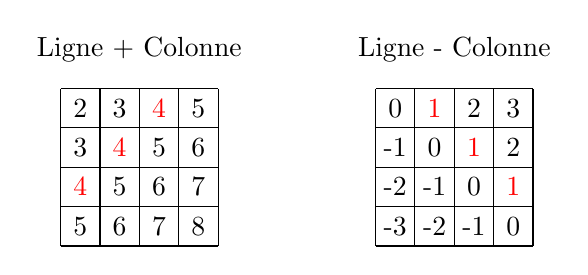
\begin{tikzpicture}[node distance=1.5em]
 \node at (1cm, 2.5cm) {Ligne + Colonne};
 \pgfpathgrid[step={\pgfpoint{.5cm}{.5cm}}]
  {\pgfpoint{0cm}{0cm}}{\pgfpoint{2cm}{2cm}}
 \pgfusepath{stroke}
 \foreach \x in {1,2,3,4} {
  \foreach \y in {1,2,3,4} {
   \pgfmathtruncatemacro{\z}{\x+5-\y};
   \ifthenelse{\z=4}{
    \def\c{red};
   }{
    \def\c{black};
   }
   \node [\c] at (\x*.5-.25, \y*.5-.25) {\z};
  }
 }

 \pgftransformxshift{4cm}
 \node at (1cm, 2.5cm) {Ligne - Colonne};
 \pgfpathgrid[step={\pgfpoint{.5cm}{.5cm}}]
  {\pgfpoint{0cm}{0cm}}{\pgfpoint{2cm}{2cm}}
 \pgfusepath{stroke}
 \foreach \x in {1,2,3,4} {
  \foreach \y in {1,2,3,4} {
   \pgfmathtruncatemacro{\z}{\x-(5-\y)}
   \ifthenelse{\z=1}{
    \def\c{red};
   }{
    \def\c{black};
   }
   \node [\c] at (\x*.5-.25, \y*.5-.25) {\z};
  }
 }
\end{tikzpicture}
\end{center}
Une diagonale est donc caractérisé par une direction et un numéro.

\Question
Ecrire un prédicat \verb$num_diag(L1,L2)$ qui sera appelé avec \verb$L1$
instancié à une liste de variables à domaine fini. Ce prédicat est vrai si la
liste \verb$L2$ représente les numéros de diagonales $\diagup$ sur lesquelles
sont les reines sachant que le plateau correspondant est donné par la liste 
\verb$L1$.
S'il est appelé avec \verb$L1 = [A,B,C]$ alors \verb$L2$ devra être instancié
à une liste de variables à domaine fini \verb$L2 = [X,Y,Z]$ tel 
\verb$X = A + 1$, \verb$Y= B + 2$ et \verb$Z = C + 3$.

\Question
Ajouter un argument à ce prédicat pour générer la liste des diagonales
$\diagdown$.

Indication : Prolog ne gère pas les contraintes sur les entiers négatifs. Il
faut donc penser à translater le numéro des diagonale $\diagdown$.

\Question
Compléter le problème des n tours pour résoudre le problème des n reines.
\end{Exercise}
\begin{CAnswer}
\begin{enumerate}
 \item \verbatiminput{diag.pro}
 \item \verbatiminput{diags.pro}
 \item \verbatiminput{n_reines.pro}
\end{enumerate}

\end{CAnswer}

\begin{Exercise}[title={Elimination des symétries}]
Il est souvent possible à partir d'une solution d'un problème en trouver
d'autres par une transformation assez simple. On dit alors que le problème
possède des symétries. On peut donc rajouter des contraintes pour éviter les
solutions symétriques et générer si nécessaire les solutions symétriques.
\Question Si un damier est solution au problème des n reines alors la symétrie
par rapport à un axe horizontal sera lui-aussi une solution. Trouvez une
propriété toujours vraie pour un plateau ou son symétrique mais jamais les 
deux à la fois.
\Question Ecrire le nouveau prédicat \verb$n_reines/2$ ne générant pas les
réponses symétriques par rapport à un axe vertical.
\Question Le problème présente aussi une symétrie selon un axe vertical.
Ecrivez un nouveau prédicat qui élimine ces solutions symétriques.

Indication : utiliser l'opérateur de division entière \verb$//$.
\end{Exercise}
\begin{CAnswer}
\begin{enumerate}
 \item Si la reine de ligne $i$ est sur la colonne $j$ et que la reine de 
       ligne $k$ est sur la colone $l$ tel que $k < l$ alors ce ne sera jamais
       vrai pour le symétrique et inversement.
 \item \verbatiminput{n_reines_sym_h.pro}
       \verb$=<$ pour le cas \verb$N = 1$
 \item On limite par exemple la première reine a être dans la moitié gauche du
       plateau,
       \verbatiminput{n_reines_sym_h_v.pro}
\end{enumerate}
\end{CAnswer}

\begin{Exercise}[title={Vérification}]
Grâce au prédicat \verb$findall/3$, vérifiez le nombre de solutions trouvées
par chacune des méthode.
\end{Exercise}
\begin{CAnswer}
\verbatiminput{decompte_solutions.pro}
\begin{verbatim}
| ?- decompte_solutions(10,N1,N2,N3).
N1 = 724
N2 = 362
N3 = 301
(160 ms) yes
\end{verbatim}
\end{CAnswer}

\begin{Exercise}[title={Et pour aller plus loin}]
En tournant le plateau de $90°$ on obtient aussi une nouvelle solution. Ecrire
un nouveau prédicat pour résoudre le problème en supprimant cette symétrie.
\end{Exercise}
\begin{CAnswer}

\end{CAnswer}

\end{document}
